\begin{center}
 \textsc{Физбой, 11 класс. Полуфинал.}
\end{center}
\vspace{0.01cm}
\hrule
\parindent=0mm

\task{Найдите частоту малых колебаний математического маятника
   относительно его нижнего положения равновесия, если непосредственно
   под равновесным положением шарика на расстоянии $h$ от него
   закреплен заряд $Q$. Длина нити $l$, масса шарика $m$, заряд $q$.}

\task{Легкая нерастяжимая нить длиной $2 \unit{м}$ удерживается за
   ее концы так, что они находятся на данной высоте рядом друг с
   другом. На нити висит проволочная скобка в виде перевернутой буквы
   U. Масса скобки равна 1 грамму. Нить выдерживает максимальную
   растягивающую силу $F = 5 \unit{Н}$ ($F \gg mg$). Концы нити
   начинают перемещать в противоположных горизонтальных направлениях с
   одинаковыми скоростями $1 \mathrm{м/с}$. В какой-то момент нить не
   выдерживает и рвется. На какую максимальную высоту в момент разрыва
   нити взлетит скобка? Сопротивлением воздуха пренебречь.}

\taskpic{Над одним молем идеального газа совершают процесс, показанный на
   рисунке. Найти максимальную температуру газа в течение этого
   процесса (процесс считать квазистатическим)}{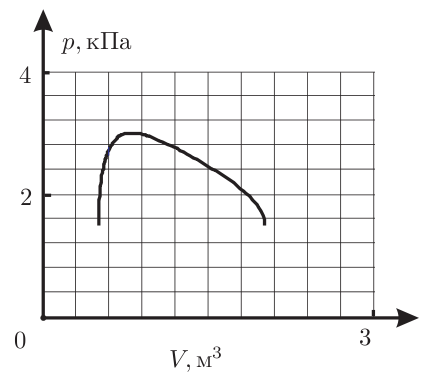
\includegraphics[width=4cm]{fb11_s_3.png}}

\taskpic{C одним молем идеального одноатомного газа провели замкнутый
цикл, изображённый на рисунке, где $1–2$ изотерма, $2–3$ изобара,
$3–4$ политропа, для которой $C = R/2$, и $4–1$ изохора. Минимальная
температура, достигаемая газом в цикле, $T_{min} = 300 \,
К$. Политропическим процессом называется процесс, происходящий с
постоянной теплоёмкостью $C$. Определите КПД цикла
$\eta$.}{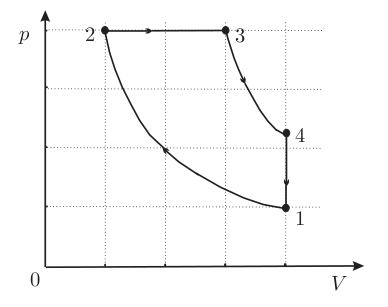
\includegraphics[width=4cm]{fb11_s_4.png}}

\task{В схеме, изображенной на рисунке, имеются четыре диода. Известно, что при любом
   напряжении, подведйнном к выводам схемы, ток через амперметр не течет. ВАХ трех диодов $D1$, $D2$ и
   $D3$ известны (см. график). Постройте ВАХ четвертого диода.
}

\taskpic{В архиве Снеллиуса найден чертеж оптической схемы. От времени чернила выцвели и на чертеже остались видны только
   три точки --- фокус линзы $F$, источник света $S$, точка $L$, принадлежащая плоскости тонкой линзы, и часть прямой линии
   а, соединяющий источник света и его изображение $S'$. Из пояснений к чертежу следует, что точка $S'$ отстоит от
   плоскости линзы на расстояние, большим, чем точка $S$.
   Возможно ли по этим данным восстановить исходную схему? Если да, то покажите, как это сделать. Чему равно
   фокусное расстояние линзы?
}{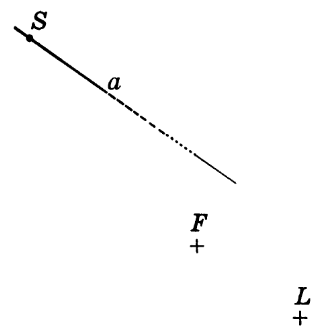
\includegraphics[width=4cm]{fb11_s_6.png}}

\begin{center}
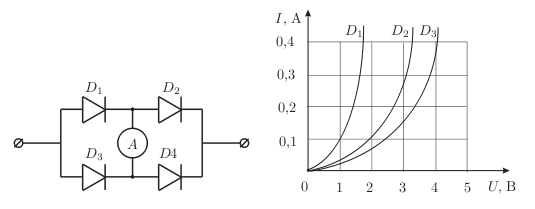
\includegraphics[width=10cm]{fb11_s_5.png}
\end{center}

\setcounter{notask}{1}

% ФИЗБОЙ, СУКА!!!
% 11 КЛАСС

% 1) Электростатика
%    Задача 6.1.14
%    Какой минимальный заряд q нужно закрепить в нижней точне сферической полости радиуса R, чтобы в
%    поле тяжести небольшой шарик массы m и заряда Q находился в верхней точке полости в положении
%    устойчивого равновесия?

%   Замена:
%    Найдите частоту малых колебаний математического маятника относительно его нижнего положения
%    равновесия, если непосредственно под равновесным положением шарика на расстоянии h от него
%    закреплен заряд Q. Длина нити l, масса шарика m, заряд q.

% еще задача 11.7 (Козел)

% 2) Динамика
%    Задача 1.17 (Проволочная скобка)
%    Легкая нерастяжимая нить длиной 2м удерживается за ее концы так, что они находятся на данной высоте рядом друг
%    с другом. На нити висит проволочная скобка в виде перевернутой буквы U. Масса скобки равна 1 грамму. Нить
%    выдерживает максимальную растягивающую силу F = 5Н. (F>>mg). Концы нити начинают перемещать в противоположных
%    горизонтальных направлениях с одинаковыми скоростями 1м/с. В какой-то момент нить не выдерживает и рвется. На
%    какую максимальную высоту в момент разрыва нити взлетит скобка? Сопротивлением воздуха пренебречь.
%    На 10 класс. Если будет совсем уныло - то и на 11ый.

%   Замена:
%    (вроде жесть) 11.84, Козел. На рисунке показана траектория движения лодки, которую
%    оттолкнули от берега рекитак, что в начальнгый момент ее скорость v0 = 1,0 м/с была
%    направлена перпендикулярно берегу. В точке С траектории лодка была через 1 с, в точке D -
%    через 2 с. Определите скорость u течения реки.

% 3) Теплогазы

%    Задача 2.9
%    Над одним молем идеального газа совершают процесс, показанный на рисунке. Найти максимальную температуру газа в
%    течение этого процесса (процесс считать квазистатическим).

%    Экспериментатор Глюк обратил внимание на то, что почти у всех известных ему изопроцессов
%    (изохорического, изобарического, изотермического и адиабатического) график зависимости
%    давления от объема имеет соответствующее название: изохора, ихобара, изотерма и адиабата.
%    У процесса же, в ходе которого не изменяется внутренняя энергия, такого названия нет! Глюк
%    решил восполнить этот пробел и назвал полученную зависимость изоэргой. Далее он решил
%    сравнить ход изоэрги с изотермой и адиабатой для реального одноатомного газа при условиях,
%    близких к нормальным. На рисунке приведены результаты его исследований. Выясните, какому из
%    трех процессов 1-2, 1-3 или 1-4 соответствует "изоэрга", какому - изотерма, а какому -
%    адиабата. Ответ обоснуйте.

%   Замена:
%    Задача 2.7
%    Оцените на какую величину (дельта)х за сутки увеличивается толщина льда, покрывающего водоем, при температуре
%    окружающей среды Т = -20С. В начале похолодания толщина льда была равна 20см. Теплопроводность льда 2.2 Вт/(м*К),
%    его удельная теплота плавления 3.35*10^5 Дж/кг, а плотность 900 кг/см^3.

% 4) Схема

%    Задача 3.7 В схеме, изображенной на рис., имеются четыре диода. Известно, что при любом
%    напряжении, подведйнном к выводам схемы, ток через амперметр не течет. ВАХ трех диодов Д1, Д2 и
%    Д3 известны (см. график). Постройте ВАХ четвертого диода.

%   Замена:

% 5) Оптика

%    11.92, 11.88, 11.54, 11.44!!!!!!!!!!!!




% ---------------------------------------------------------------------------------------------------------------------
% 1) Какой минимальный заряд q нужно закрепить в нижней точне сферической полости радиуса R, чтобы в
%    поле тяжести небольшой шарик массы m и заряда Q находился в верхней точке полости в положении
%    устойчивого равновесия?

% 2) Легкая нерастяжимая нить длиной 2м удерживается за ее концы так, что они находятся на данной высоте рядом друг
%    с другом. На нити висит проволочная скобка в виде перевернутой буквы U. Масса скобки равна 1 грамму. Нить
%    выдерживает максимальную растягивающую силу F = 5Н. (F>>mg). Концы нити начинают перемещать в противоположных
%    горизонтальных направлениях с одинаковыми скоростями 1м/с. В какой-то момент нить не выдерживает и рвется. На
%    какую максимальную высоту в момент разрыва нити взлетит скобка? Сопротивлением воздуха пренебречь.

% 3) Над одним молем идеального газа совершают процесс, показанный на рисунке. Найти максимальную температуру газа в
%    течение этого процесса (процесс считать квазистатическим).

% 4) Оцените на какую величину (дельта)х за сутки увеличивается толщина льда, покрывающего водоем, при температуре
%    окружающей среды Т = -20С. В начале похолодания толщина льда была равна 20см. Теплопроводность льда 2.2 Вт/(м*К),
%    его удельная теплота плавления 3.35*10^5 Дж/кг, а плотность 900 кг/см^3.

% 5) В схеме, изображенной на рис., имеются четыре диода. Известно, что при любом
%    напряжении, подведйнном к выводам схемы, ток через амперметр не течет. ВАХ трех диодов Д1, Д2 и
%    Д3 известны (см. график). Постройте ВАХ четвертого диода.

% 6) В архиве Снеллиуса найден чертеж оптической схемы. От времени чернила выцвели и на чертеже остались видны только
%    три точки - фокус линзы F, источник света S, точка L, принадлежащая плоскости тонкой линзы, и часть прямой линии
%    а, соединяющий источник света и его изображение S'. Из пояснений к чертежу следует, что точка S' отстоит от
%    плоскости линзы на расстояние, большим, чем точка S.
%    Возможно ли по этим данным восстановить исходную схему? Если да, то покажите, как это сделать. Чему равно
%    фокусное расстояние линзы?
% -----------------------------------------------------------------------------------------------------------------------

% Замены:
% 1) Найдите частоту малых колебаний математического маятника относительно его нижнего положения
%    равновесия, если непосредственно под равновесным положением шарика на расстоянии h от него
%    закреплен заряд Q. Длина нити l, масса шарика m, заряд q.

% 2) На рисунке показана траектория движения лодки, которую
%    оттолкнули от берега рекитак, что в начальнгый момент ее скорость v0 = 1,0 м/с была
%    направлена перпендикулярно берегу. В точке С траектории лодка была через 1 с, в точке D -
%    через 2 с. Определите скорость u течения реки.

% 3) Экспериментатор Глюк обратил внимание на то, что почти у всех известных ему изопроцессов
%    (изохорического, изобарического, изотермического и адиабатического) график зависимости
%    давления от объема имеет соответствующее название: изохора, ихобара, изотерма и адиабата.
%    У процесса же, в ходе которого не изменяется внутренняя энергия, такого названия нет! Глюк
%    решил восполнить этот пробел и назвал полученную зависимость изоэргой. Далее он решил
%    сравнить ход изоэрги с изотермой и адиабатой для реального одноатомного газа при условиях,
%    близких к нормальным. На рисунке приведены результаты его исследований. Выясните, какому из
%    трех процессов 1-2, 1-3 или 1-4 соответствует "изоэрга", какому - изотерма, а какому -
%    адиабата. Ответ обоснуйте.

% 4) В чайник с нагревательным элементом мощностью Р = 2200 Вт налили V1 = 1,5л холодной воды и включили
%    его. когда вода закипела, он автоматически отключился. Через t1 = 60с его снова включили, а еще через t2 = 6с
%    вода закипела и чайник выключился. сразу после этого его еще раз включили, но сняв крышку. Автоматический
%    выключатель, срабатывающий под давлением пара, перестал действовать, и вода из чайника начала выкипать. Через
%    t3 = 240с после последнего включения измерили объем оставшейся воды. Он оказался равным V2 = 1,3л. Каково
%    значение удильной теплоты парообразования воды r? Удельная теплоемкость воды с = 4200 Дж/(кг*К), плотность
%    р = 1000 кг/м^3. Теплоемкостью чайника пренебречь.

% 5) Имеется батарейка с ЭДС Е1 и внутренним сопротивлением r1, а также некоторое количество одинаковых батареек
%    с эдс Е2 = Е1/2. Если последовательно с батареей Е1 подключить некоторое количество батареек Е2 и нагрузку, то
%    сила тока в цепи при любом количестве батареек Е2 будет одинаковой. Если же к батарейке Е1 параллельно
%    подсоединить любое число батареек Е2 и ту же нагрузку, то сила тока через нее останется равной прежнему
%    значению. Полярности всех батарей считать одинаковыми. Найдите сопротивление нагрузки R, а также внутреннее
%    сопротивление r2 батареек Е2.

% 6) Говорят, что в архиве Снеллиуса нашли оптическую схему, на которой были изображены линза, предмет - палочка
%    длины l и ее изображение длины l'. От времени чернила выцвели, и остались видны только две точки: вершина
%    палочки S и ее изображение S'. Из текста следовало, что главная оптическая ось проходила через середину палочки
%    перпендикулярно ей. Определите построением положения линзы, главной оптической оси, фокусов линзы, предмета и
%    его изображения и укажите, какая это линза (собирающая или рассеивающая), если l = 5см, l' = 2см, SS' = 15см.
